\subsection{Reporting}

\subsubsection{Scope}
\par{The reporting module allows for better control and understanding of what has been done and what still needs to be done as well as the time constraints that apply to all tasks and the overall schedule.}

\begin{figure}[h]
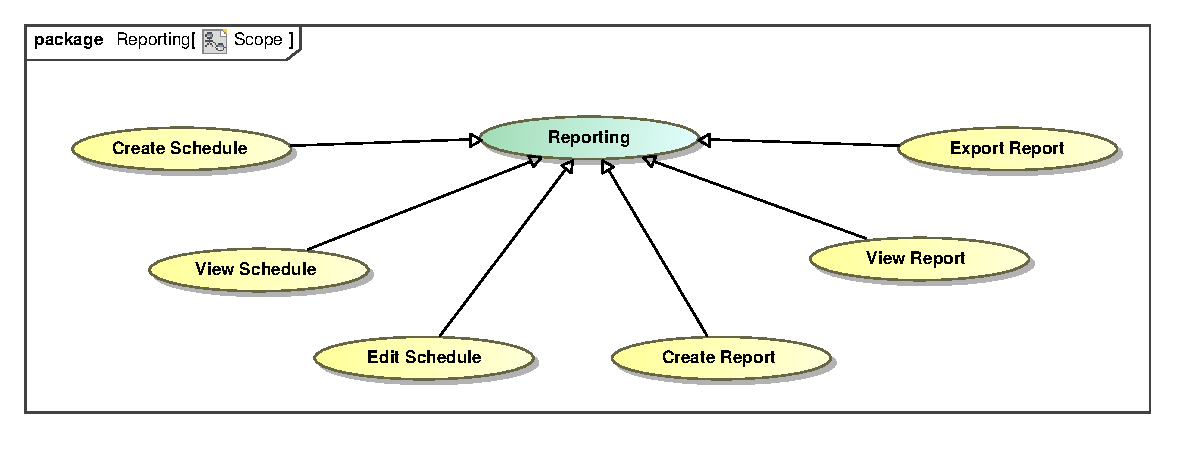
\includegraphics[height=200px, width=500px]{epsImages/Reporting/ReportScope.eps}
\caption{Scope for reporting module}
\end{figure}

\subsubsection{Use Cases}

\begin{enumerate}
\item \textbf{Create Schedule - priority: critical}
\par{This use case allows a user to create a work schedule for the book that may consist of multiple tasks, so as to facilitate concurrent work(Tasks).}
\textbf{Service Contract:} 
\begin{figure}[h]
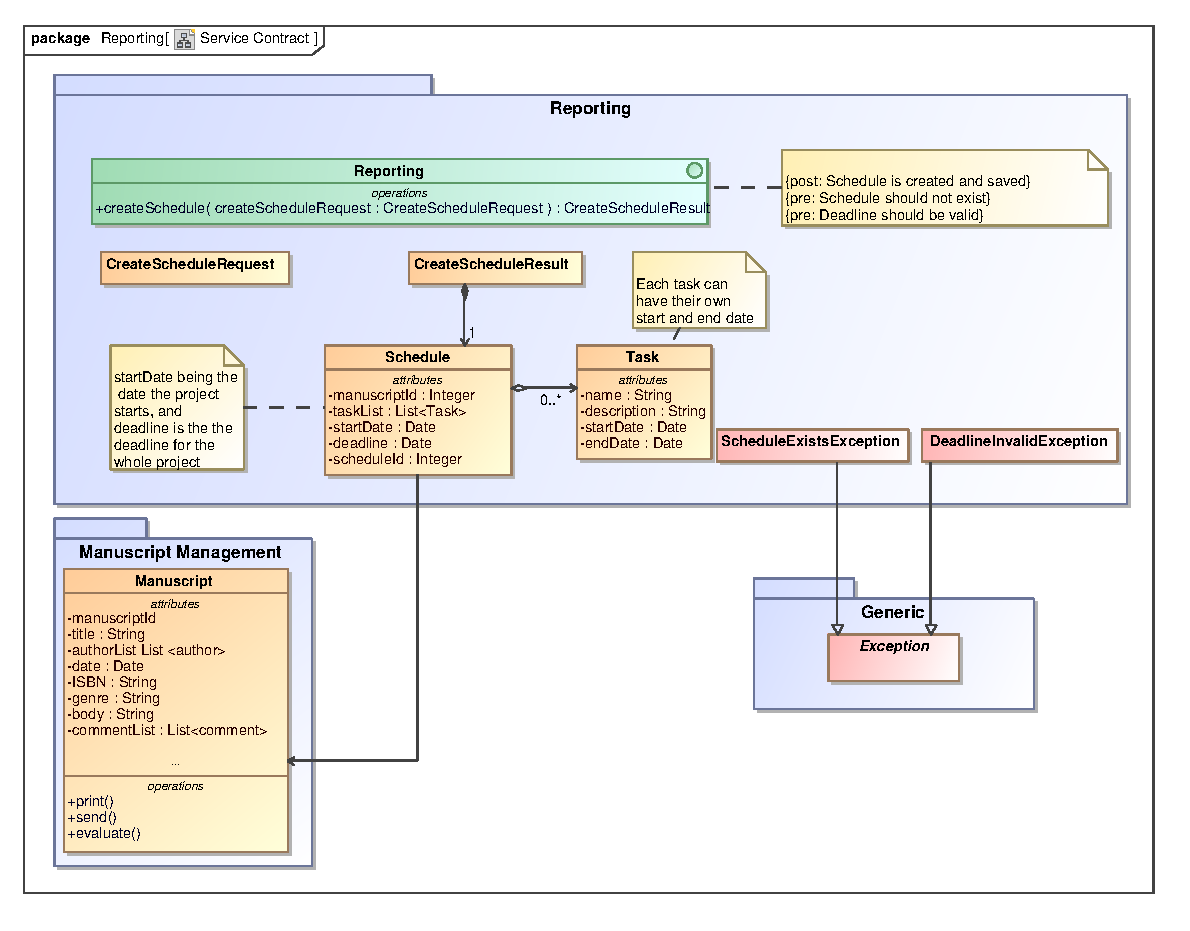
\includegraphics[height=200px, width=500px]{epsImages/Reporting/createSchedule.eps}
\caption{Service contract for creating a work schedule}
\end{figure}
\newpage

\item \textbf{View Schedule - priority: critical}
\par{This use case allows a user to view the work schedule for the book.}\\
\textbf{Service Contract:} 
\begin{figure}[h]
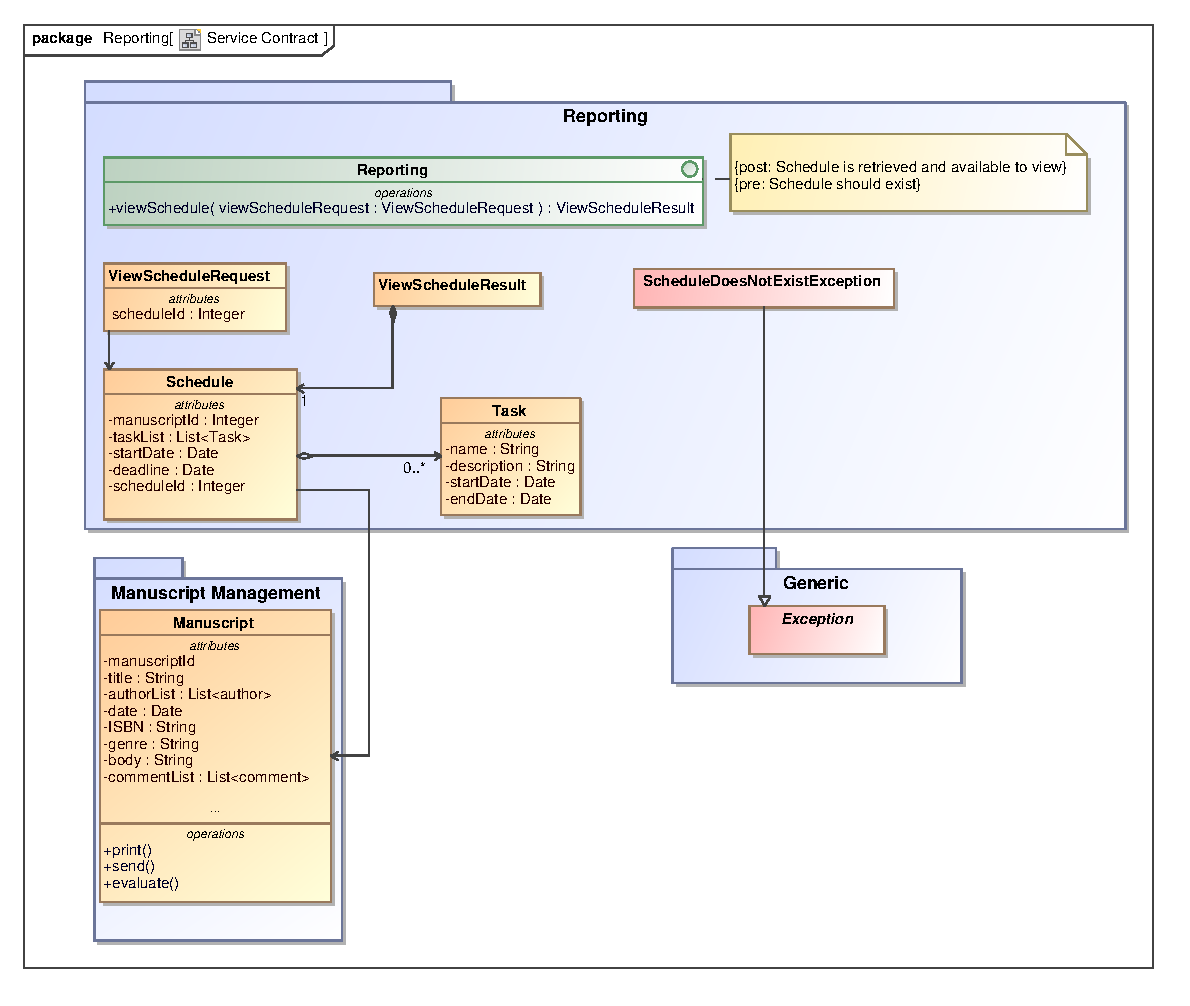
\includegraphics[height=200px, width=500px]{epsImages/Reporting/viewSchedule.eps}
\caption{Service contract for viewing a work schedule}
\end{figure}


\item \textbf{Edit Schedule - priority: critical}
\par{This use case allows a user to make changes to the work schedule of the book.}\\
\textbf{Service Contract:} 

\begin{figure}[h]
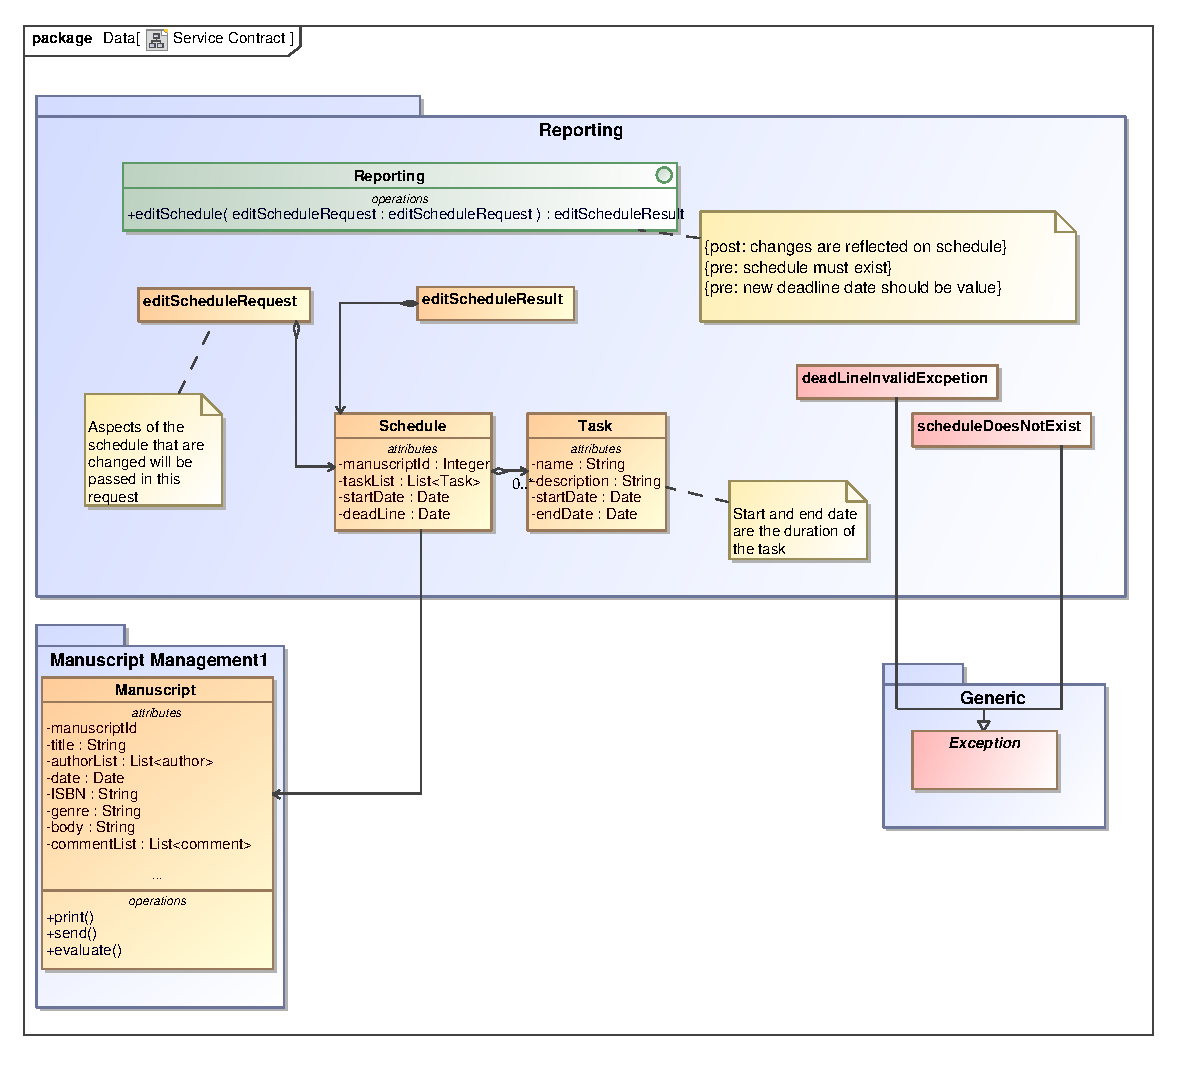
\includegraphics[height=200px, width=500px]{epsImages/Reporting/editSchedule.eps}
\caption{Service contract for editing a work schedule}
\end{figure}
\newpage

\item\textbf{Create Report - priority: important}
\par{This use case creates a report based on filters, therefore allowing it to be in printable format.}\\
\textbf{Service Contract:} 

\begin{figure}[h]
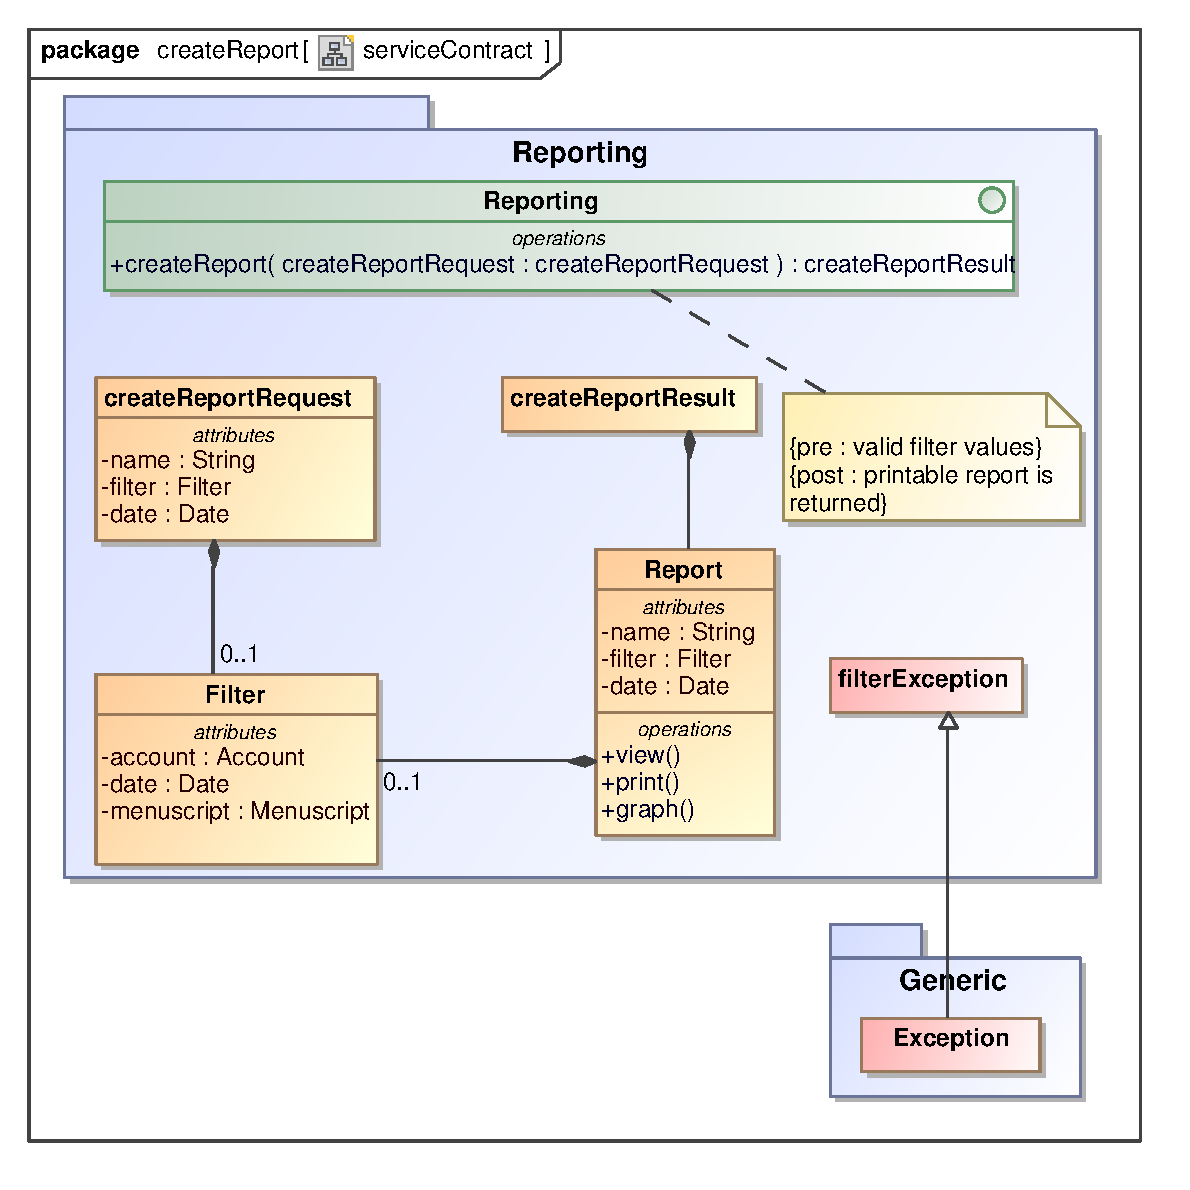
\includegraphics[height=200px, width=500px]{epsImages/Reporting/createReport.eps}
\caption{Service contract for creating a report}
\end{figure}


\item \textbf{View Report - priority: important}
\par{This use case allows users to view a generated report, on the system (before exporting to say, a pdf for example).}\\
\textbf{Service Contract:} 

\begin{figure}[h]
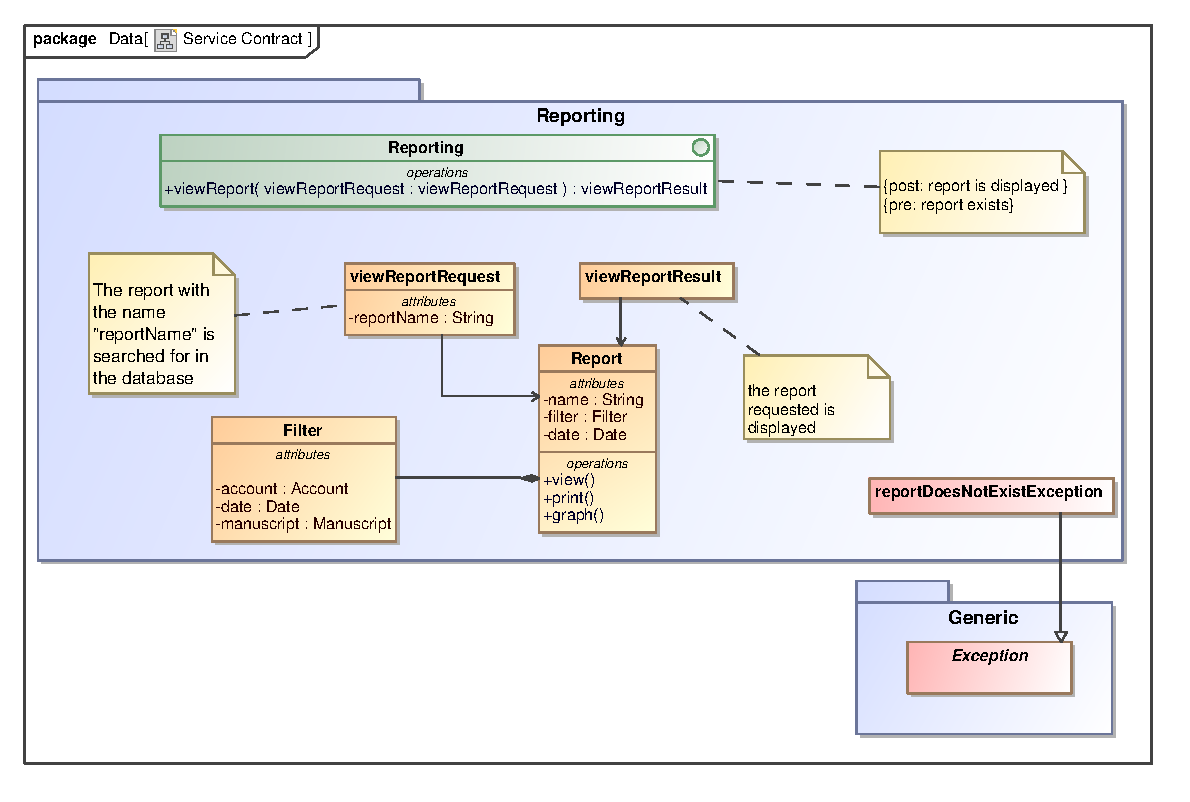
\includegraphics[height=200px, width=500px]{epsImages/Reporting/viewReportServiceContract.eps}
\caption{Service contract for viewing a report}
\end{figure}
\newpage

\item \textbf{Export Report - priority: important}
\par{This use case which allows one to export a manuscript}\\
\textbf{Service Contract:} 

\begin{figure}[h]
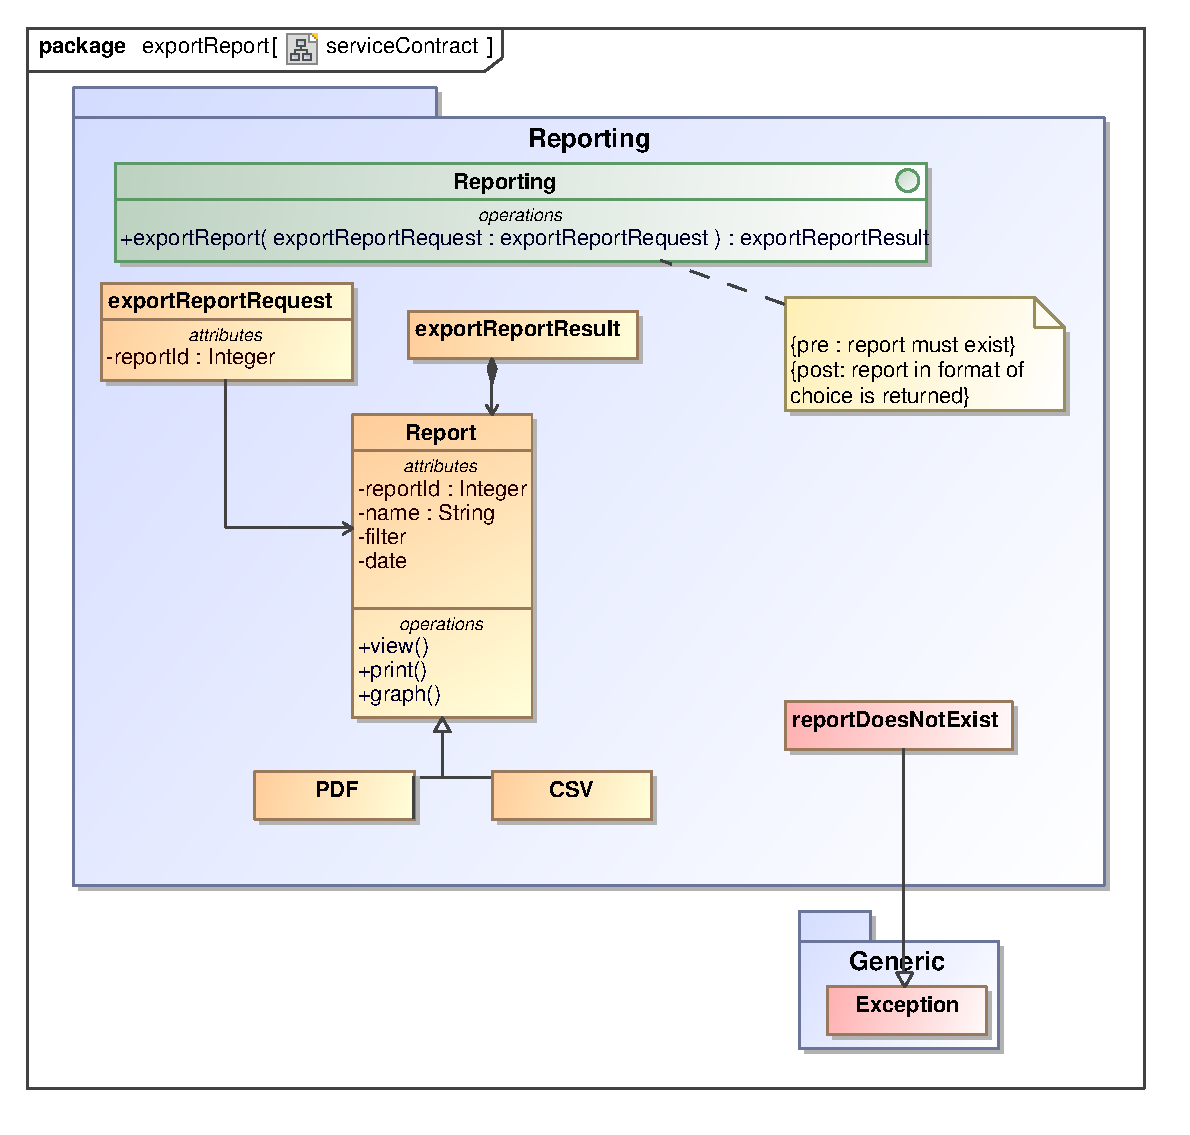
\includegraphics[height=200px, width=500px]{epsImages/Reporting/exportReport.eps}
\caption{Service contract for exporting a report}
\end{figure}


\subsubsection{Domain Model}
\par{The reporting module is responsible for keeping track of all task, schedules and progress. A schedule class is setup to consist of various tasks, starting with none and they can be added over time. The overall schedule has a starting and a deadline date, while the inner tasks also consist of their own unique start and end dates. A report can be generated by using a user specified filter that can consist of multiple fields.}

\begin{figure}[h]
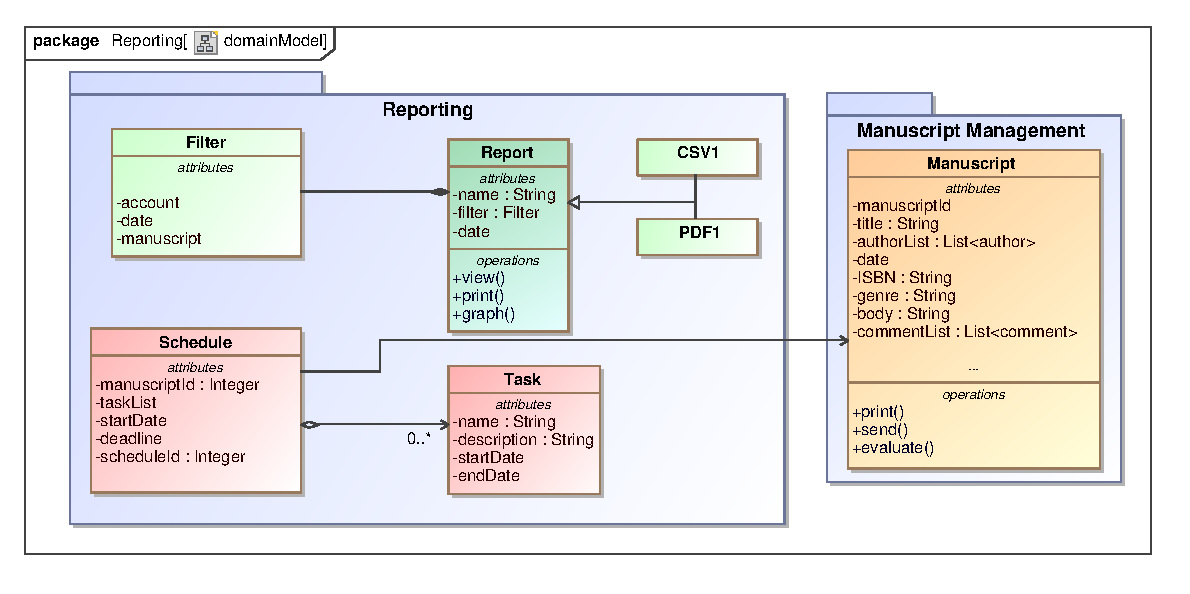
\includegraphics[height=200px, width=500px]{epsImages/DomainModels/Reporting.eps}
\caption{The domain model for the reporting module.}
\end{figure}
\newpage

\end{enumerate}

